76. \begin{figure}[ht!]
\center{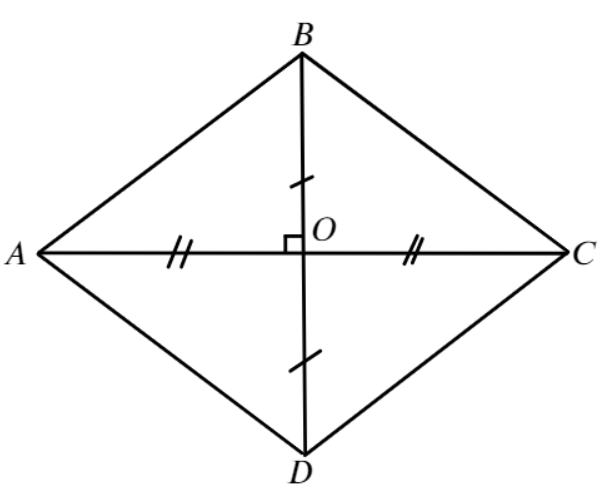
\includegraphics[scale=0.35]{g8-76.png}}
\end{figure}\\
В ромбе диагонали перпендикулярны и делятся (как и в любом параллелограмме) точкой пересечения пополам. Пусть $BD=12,$ тогда $BO=12:2=6$ и по теореме Пифагора $AO=\sqrt{AB^2-BO^2}=\sqrt{100-36}=8,$ значит $AC=2AO=16.$\\
